\section{BJT's logic gate application}
Figure \ref{lab3_notGate_de} describes a straightforward NOT gate theoretical implementation using an NPN bipolar junction transistor. In the circuit, the NPN junction transistor operates in the saturation mode.

\begin{figure}[H]
    \centering
    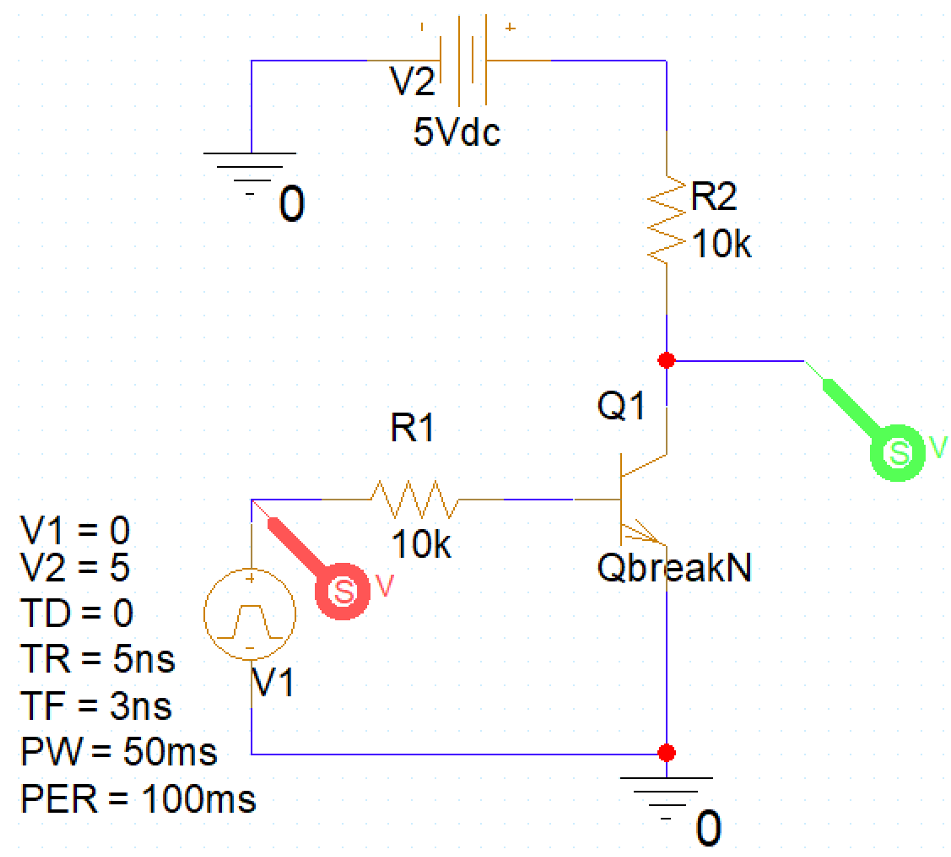
\includegraphics[width=10cm]{graphics/ex12/f1.png}
    \caption{NPN theoretical NOT gate}
    \label{lab3_notGate_de}
\end{figure}

V1 = 0  When the source is off, the voltage would be 0V.\\
V2 = 5  When the source is on, the voltage would be 5V.\\
TD = 0  Delay time. This exercise assumes that there is no delay.\\
TR = 5ns  The rise time of the pulse (from off to on stage).\\
TF = 3ns  The fall time of the pulse (from on to off stage).\\
PW = 50ms  Pulse width: The time in which the source keeps on.\\
PER = 100ms  The period of the signal.\\

\textbf{\textit{Tips:}}\\
\\
To get the Voltage Pulse Source component in the PSpice for TI, go to \textbf{\textit{Place -> Pspice Compoment... -> Source -> Voltage Sources -> Pulse.}}

\newpage
\textbf{\textit{Your image goes here:}}\\

\begin{figure}[H]
    \centering
    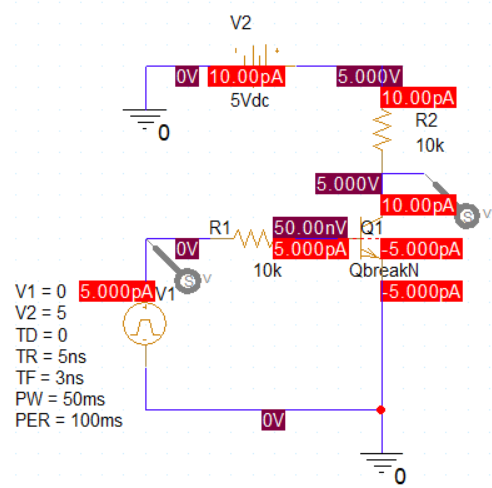
\includegraphics[width=\linewidth]{graphics/ex12/f2.png}
    \caption{NPN NOT gate simulation}
\end{figure}
